\documentclass[12pt,a4paper]{report}

%----------------------------------------------------------------------------------------
%   PACKAGES
%----------------------------------------------------------------------------------------
\usepackage[francais]{babel} % French language package
\usepackage[utf8]{inputenc} % UTF8
\usepackage[T1]{fontenc} % acute french accents
\usepackage[pdftex]{graphicx} % figures
\usepackage{hyperref} % hyperlinks
\usepackage[dvipsnames]{xcolor} % colors
\usepackage{amsthm} % mathematical symbols
\usepackage{natbib} % To add the bibligraphy
\usepackage[page,toc,titletoc,title]{appendix} %To add appendices to the document
\usepackage[nottoc,notlot,notlof]{tocbibind} %To bind the table of contents to the bibligoraphy
\usepackage{titlesec}
\titleformat{\chapter}[display]
{\normalfont\huge\bfseries}{\chaptertitlename\ \thechapter}{20pt}{\Huge}
\titlespacing*{\chapter}{0pt}{-50pt}{40pt}

\makeatletter
\setlength{\@fptop}{0pt}
\makeatother

\hypersetup{
    colorlinks,
    linkcolor={red!50!black},
    citecolor={blue!50!black},
    urlcolor={blue!80!black}
}

\newcommand{\HRule}{\rule{\linewidth}{0.5mm}} % Defines a new command for the horizontal lines

\theoremstyle{definition}
\newtheorem*{definition}{Définition}
\newtheorem{example}{Exemple}
\newtheorem*{remark}{Remarque}

\begin{document}
\pagenumbering{roman}
%----------------------------------------------------------------------------------------
%   TITLE PAGE
%----------------------------------------------------------------------------------------
\begin{titlepage}
\center

%----------------------------------------------------------------------------------------
%   LOGOS SECTION
%----------------------------------------------------------------------------------------

\includegraphics[scale=0.5]{images/umLogo.png} % Université de Montpellier Logo
\hspace{\fill}

\includegraphics[scale=0.25]{images/fdsLogo.jpg} % Faculté de Sciences Logo

%----------------------------------------------------------------------------------------
%   HEADING SECTIONS
%----------------------------------------------------------------------------------------
\textsc{\LARGE M1 Informatique AIGLE}\\[1cm]
\textsc{\Large \textbf{HMIN201}}\\[0.25cm]
\textsc{\large M1 TER}\\[0.5cm]

%----------------------------------------------------------------------------------------
%   TITLE SECTION
%----------------------------------------------------------------------------------------
\HRule \\[0.4cm]
{ \huge \bfseries TER: Software Heritage}\\[0.4cm]
{ \Large \bfseries Rapport Final}\\[0.4cm]
\HRule \\[0.5cm]

%----------------------------------------------------------------------------------------
%   AUTHORS AND SUPERVISORS SECTION
%----------------------------------------------------------------------------------------
{ \huge \bfseries Groupe \textsc{Bajonim}}\\[0.4cm]
\begin{minipage}{0.4\textwidth}
\centering \small
\textbf{Bachar \textsc{Rima}}, \\ \href{mailto:bachar.rima@etu.umontpellier.fr}{bachar.rima@etu.umontpellier.fr}\\ % Student
\textbf{Joseph \textsc{Saba}}, \\ \href{mailto:joseph.saba@etu.umontpellier.fr}{joseph.saba@etu.umontpellier.fr}\\ % Student
\textbf{Tasnim \textsc{Shaqura}}, \\ \href{mailto:tasnim.shaqura@etu.umontpellier.fr}{tasnim.shaqura@etu.umontpellier.fr}\\ % Student
\end{minipage} \\[0.8cm]

\begin{minipage}[b]{0.4\textwidth}
\begin{flushleft} \large
\emph{Encadrant:} \\
Jessie \textsc{Carbonnel} % Academic Supervisor
\end{flushleft}
\end{minipage}
~
\begin{minipage}[b]{0.4\textwidth}
\begin{flushright} \large
\emph{Responsable de l'UE:} \\
Mattieu \textsc{Lafourcade} % UE Supervisor
\end{flushright}
\end{minipage}\\[1.5cm]

%----------------------------------------------------------------------------------------
%   DATE SECTION
%----------------------------------------------------------------------------------------
{\large 27 mai 2019}\\[1cm]
\hspace{\fill}
\vfill % Fill the rest of the page with whitespace
\end{titlepage}

%----------------------------------------------------------------------------------------
%   INTRODUCTION
%----------------------------------------------------------------------------------------
\tableofcontents
\cleardoublepage

\pagenumbering{arabic}
\setcounter{page}{1}
\chapter{Introduction}
Les logiciels sont actuellement omniprésents dans tous les aspects de notre vie quotidienne; ils constituent l'un des piliers de l'héritage humain et doivent être préservés contre toute suppression et tout endommagement. Archiver leurs codes source s'avère ainsi une tâche primordiale. En effet, le code source d’un logiciel constitue un artefact logiciel essentiel dans le domaine des connaisances scientifiques, culturelles, et techniques. D’autre part, le code source est facilement lisible et compréhensible par les humains, et peut être transformé en fichiers exécutables. À ce titre là, des plateformes ont déjà été proposées telles que \href{https://archive.org/}{\texttt{The Internet Archive}} et \href{https://unescopersist.org/}{\texttt{UNESCO Persist}}. Toutefois, ces plateformes se concentraient plutôt sur la préservation des fichiers exécutables au lieu du code source \textsuperscript{\citep{internetArchive}}\textsuperscript{\citep{unescoPersist}}.

\section{Description de Software Heritage}
\texttt{Software Heritage} est une initiative lancée par \textbf{INRIA}\textcolor{RoyalBlue}{\footnote{\textbf{Institut National de Recherche en Informatique et Automatique}}}, soutenue par l'\textbf{UNESCO} et visant \og la collecte, la conservation et le partage de code source de tous les logiciels publiquement accessibles depuis n'importe quelle plateforme d'hébergement de code source \fg \textsuperscript{\citep{dicosmoWhyAndHow}}.

Son architecture consiste en un \textit{framework} permettant de retrouver le code source des logiciels susmentionnés et de les ingérer au sein de l’archive universel de \texttt{Software Heritage}. En particulier, les \textbf{Listers} en constituent une partie centrale: il s’agit de \textit{crawlers} configurés pour parcourir des dépôts de code source, \og \textit{mapper} \fg~ leurs modèles à des modèles intégrables à l'infrastructure, et reporter l'ingestion de leur contenu à d’autres composants du \textit{framework}. L'ingestion du contenu d'un dépôt \og \textit{listé} \fg au sein de l'archive est effectuée par des composants spécifiques, les \textbf{Loaders}. Enfin, la planification des tâches du \textit{listing} et du \textit{loading} est régulée par un \textbf{Scheduler}, un composant interagissant avec une queue de tâches asynchrones opérée par un serveur \texttt{Celery}.

Il faut préciser que les plateformes d’hébergement embarquent chacune des dépôts de code source à structures différentes, ce qui nécessite la création d’un \textbf{Lister} dédié pour chaque plateforme. Par ailleurs, les différentes versions d'un logiciel et leurs métadonnées associées sont gérées par un gestionnaire de version, ce qui nécessite la création d'un \textbf{Loader} dédié pour chaque gestionnaire. Actuellement, tous les \textbf{Listers} et \textbf{Loaders} ont été créés uniquement par l’équipe de \texttt{Software Heritage}. Les \textbf{Listers} développés l'ont été pour les plateformes d’hébergement les plus populaires (\texttt{Github}, \texttt{Bitbucket}, $\dots$). De même, les \textbf{Loaders} développés l'ont été pour les gestionnaires de version les plus populaires (\texttt{Git}, \texttt{SVN}, \texttt{Mercurial}, $\dots$).

\section{Contexte du TER}
Dans le cadre de ce projet, encadré par Jessie Carbonnel, du module \textbf{HMIN201} désignant le TER, encadré par Mathieu LaFourcade, notre objectif final consiste à créer un \textbf{Lister} pour une plateforme de développement ciblée. Ainsi, les tâches nécessaires à effectuer afin d'accomplir ce but peuvent être énumérées de la manière suivante :
\begin{itemize}
	\item Lire et comprendre les articles et tutoriels écrits par l’équipe de \texttt{Software Heritage} ;
	\item Analyser différentes plateformes d’hébergement afin d’en cibler une ;
	\item Concevoir et développer un \textbf{Lister} pour la plateforme choisie ;
	\item Répliquer localement l’environnement de \texttt{Software Heritage} afin de tester le \textbf{Lister} développé ;
	\item Faire une \textit{Pull Request} afin d’intégrer le \textbf{Lister} testé au dépôt de développement de \texttt{Software Heritage} sur \texttt{GitHub}.
\end{itemize}

\section{Plan du rapport}
Nous commençons ce rapport par une courte description de \texttt{Software Heritage}, suivie par la spécification du contexte du stage. Ensuite, nous détaillerons la problématique générale traitée par \texttt{Software Heritage} et la sous-problématique particulière adressée par notre projet.

Par la suite, nous fournirons une explication technique détaillée de l'infrastructure de \texttt{Software Heritage} et de son fonctionnement, l'étape fondamentale sur laquelle se base notre méthodologie, et nous terminerons la section par le planning prévisionnel du projet. Après, nous élaborerons nos approches pour la conception d'un \textbf{Lister} et son implémentation, ainsi que les résultats obtenus.

Pour conclure, nous comparerons les versions prévisionnelle et finale du planning, puis nous discuterons les difficultés rencontrées et les perspectives du projet. Finalement, nous listerons un bilan du projet en citant ses apports.

\chapter{Problématique}
\section{La diaspora du code source}

\section{La fragilité du code source}

\section{Software Heritage en tant que solution}
	Current status et roadmap de SWH

\section{Notre contribution}

\chapter{Analyse}
\section{Terminologie et fonctionnement de Software Heritage}
\subsection{Modèle des données}
Le modèle des données de \texttt{Software Heritage} est centré sur la notion de stockage d'\og \textbf{artefacts logiciels} \fg~ et leurs \textbf{informations de provenance} correspondantes, hébergés sur des \textbf{plateformes d'hébergement de code source}\textsuperscript{\citep{dicosmoWhyAndHow}}.

\subsubsection{Plateformes d'hébergement de code source}
Les \textbf{plateformes d'hébergement de code source} sont destinées à être \og \textit{crawlées} \fg~ par des \textbf{Listers} et ingérées au sein de l'archive universel de \texttt{Software Heritage} par des \textbf{Loaders}\textsuperscript{\citep{dicosmoWhyAndHow}}. Ces plateformes sont catégorisées de la manière suivante :
\begin{description}
	\item [\textit{forges} de développement collaboratif :] \texttt{GitHub}, \texttt{GitLab}, \texttt{BitBucket}, $\dots$
	\item [dépôts d'un gestionnaire de paquets :] \texttt{PyPI}\footnote{\textbf{\textit{Python Package Index}}}, \texttt{CPAN}\footnote{\textbf{\textit{Comprehensive Perl Archive Network}}}, \texttt{npm}\footnote{\textbf{\textit{Node Package Manager}}}, $\dots$
	\item [distributions logicielles FOSS\footnotemark :]\footnotetext{\textbf{\textit{Free and Open-Source Software}}} \texttt{Debian}, \texttt{Fedora}, \texttt{FreeBSD}, $\dots$
	- other types: e.g.
	\item [autres :] par exemple les \textbf{URL}s\footnote{\textbf{\textit{Uniform Resource Locator}}} personnelles et celles désignant des collections de projets institutionnels non hébergées sur des \textit{forges}.
\end{description}

\subsubsection{Artefacts logiciels}
\begin{definition}[\textbf{Artefact Logiciel}]\mbox{}\\
Selon \href{http://www.granddictionnaire.com/ficheOqlf.aspx?Id_Fiche=8367467}{Le grand dictionnaire terminologique}, un \textbf{artefact logiciel} désigne tout \og \textit{module d'information utilisé ou produit lors de la conception d'un logiciel} \fg.
\end{definition}

Dans le cadre de \texttt{Software Heritage}, pour tout logiciel hébergé sur une plateforme d'hébergement de code source, il existe plusieurs \textbf{artefacts logiciels} qui sont assez récurrent lors du développement du logiciel, et qui constituent les composants de base de l'archive\textsuperscript{\citep{dicosmoWhyAndHow}}. Ces artefacts peuvent être catégorisés de la manière suivante :
\begin{enumerate}
	\item \textit{file contents} ou \textit{blobs} ;
	\item \textit{directories} ;
	\item \textit{revisions} ou \textit{commits} ;
	\item \textit{releases} ou \textit{tags}.
\end{enumerate}

\begin{definition}[\textbf{Blob}]\mbox{}\\
Le \textbf{contenu binaire du code source} (\textit{i.e. les octets}), sans aucune métadonnée associée (même pas le nom du blob). C'est Un artefact récurrent à travers différentes versions d'un même logiciel, différents répertoires du même projet, voire même différents projets.
\end{definition}

\begin{definition}[\textbf{Directory}]\mbox{}\\
Une \textbf{liste récursive d'entrées nommées} pointant vers d'autres aretfacts (\textit{i.e. des blobs ou d'autres directories}). C'est Un artefact associé à des métadonnées divers (\textit{e.g. bits de permission, estampilles de modification, $\dots$}).
\end{definition}

\begin{definition}[\textbf{Revision}]\mbox{}\\
Une \textbf{version du \textit{directory} racine du logiciel} tel qu'il est capturé par un \textbf{gestionnaire de version} (\textit{i.e. un commit}), contenant la totalité du \textbf{code source} du projet désigné par le logiciel. C'est un artefact associé à des métadonnées divers (\textit{e.g. message de commit, estampilles, versions précédentes, $\dots$}).
\end{definition}

\begin{definition}[\textbf{Release}]\mbox{}\\
Une \textbf{revision stable} qui pourra être mise en production (\textit{i.e. un project milestone}). C'est un artefact associé à des métadonnées divers désignant les \textbf{métadonnées d'une revision} et d'autres (\textit{e.g. nom du release, version du release, signatures digitales, $\dots$}).
\end{definition}

\subsubsection{Informations de provenance des données}
Dans le cadre de \texttt{Software Heritage}, pour tout logiciel hébergé sur une plateforme d'hébergement de code source, les \textbf{informations retournées} par le \textit{crawling} de celui-ci sont appelées les informations de provenance (\textit{provenance information})\textsuperscript{\citep{dicosmoWhyAndHow}}. Ces informations peuvent être catégorisées de la manière suivante :
\begin{enumerate}
	\item \textit{software origins} ;
	\item \textit{projects} ;
	\item \textit{snapshots} ;
	\item \textit{visits}.
\end{enumerate}

\begin{definition}[\textbf{Software Origin}]\mbox{}\\
Un \textbf{ensemble de références} pointant vers les endroits de récupération des \textbf{artefacts logiciels} d'un logiciel, archivés dans \texttt{Software Heritage}. Il s'agit d'une \textbf{paire} $<$\emph{type}, \emph{url}$>$ :
\begin{description}
	\item [type :] le \textbf{type de l'origine} (un \textbf{gestionnaire de version} tel que \texttt{Git} ou \texttt{SVN}, un \textbf{paquet source} tels que \texttt{DSC}\footnote{\textbf{\textit{Debian Source Control}}}, $\dots$)
	\item [url :] une \textbf{adresse URL canonique} désignant l'\textbf{adresse de l'origine} (une \textbf{adresse clonable} par un \textbf{gestionnaire de version}, ou \textbf{téléchargeable} telle qu'un \textit{tarball} téléchargé via \texttt{wget}).
\end{description}
\end{definition}

\begin{definition}[\textbf{Project}]\mbox{}\\
Une \textbf{entité abstraite} associée à des \textbf{software origins} divers, avec leurs métadonnées correspondantes. De plus, un projet peut être \textbf{versionné} et \textbf{imbriqué} dans une \textbf{hiérarchie de projets}, et permet de générer des \textbf{ressources de développement} (\textit{e.g. websites, issue trackers, mailing lists, software origins, $\dots$}).
\end{definition}

\begin{definition}[\textbf{Snapshot}]\mbox{}\\
Une \textbf{snapshot à un instant donné} d'un/plusieurs \textbf{point(s) d'entrée} d'un logiciel référencé par un \textbf{software origin} :
\begin{itemize}
	\item s'il s'agit d'un \textbf{gestionnaire de version} : \textbf{points d'entrée} = les \textbf{branches} de développement (\textit{e.g. une snapshot de la branche principale, une autre snapshot de la branche de features $\dots$}) ;
	\item s'il s'agit d'une \textbf{distribution de paquets source} : \textbf{points d'entrée} = les \textbf{suites}\footnote{différents niveaux de maturité d'un paquet source logiciel} de développement (\textit{e.g. une snapshot pour la dernière version d'un paquet source pour la suite stable}).
\end{itemize}
\end{definition}

\begin{definition}[\textbf{Visit}]\mbox{}\\
Un \textbf{lien} entre un \textbf{software origin} et une \textbf{snapshot}, créé lors de la consultation du \textbf{software origin}, permettant d'enregistrer le \textbf{moment de son consultation} et un \textbf{snapshot entier} de son état.
\end{definition}

\subsubsection{Structure de données}
La structure de données à utiliser pour implanter l'archive doit permettre la déduplication de certains \textbf{artefacts logiciels} et \textbf{informations de provenance} tels que les \textbf{blobs}, les \textbf{directories}, les \textbf{revisions}, les \textbf{releases} et les \textbf{snapshots}. Cette déduplication est essentielle afin d'assurer une préservation à long terme et un stockage efficace. Pour ce faire, \texttt{Software Heritage} ont adopté le modèle d'un \textbf{graphe orienté acyclique Merkel}\textsuperscript{\citep{dicosmoWhyAndHow}} ou \textbf{Merkel DAG}\footnote{\textbf{\textit{Direct Acyclic Graph}}} (cf. Figure \ref{fig:swh_data_structure}).

\begin{figure}[!ht]
	\centering
	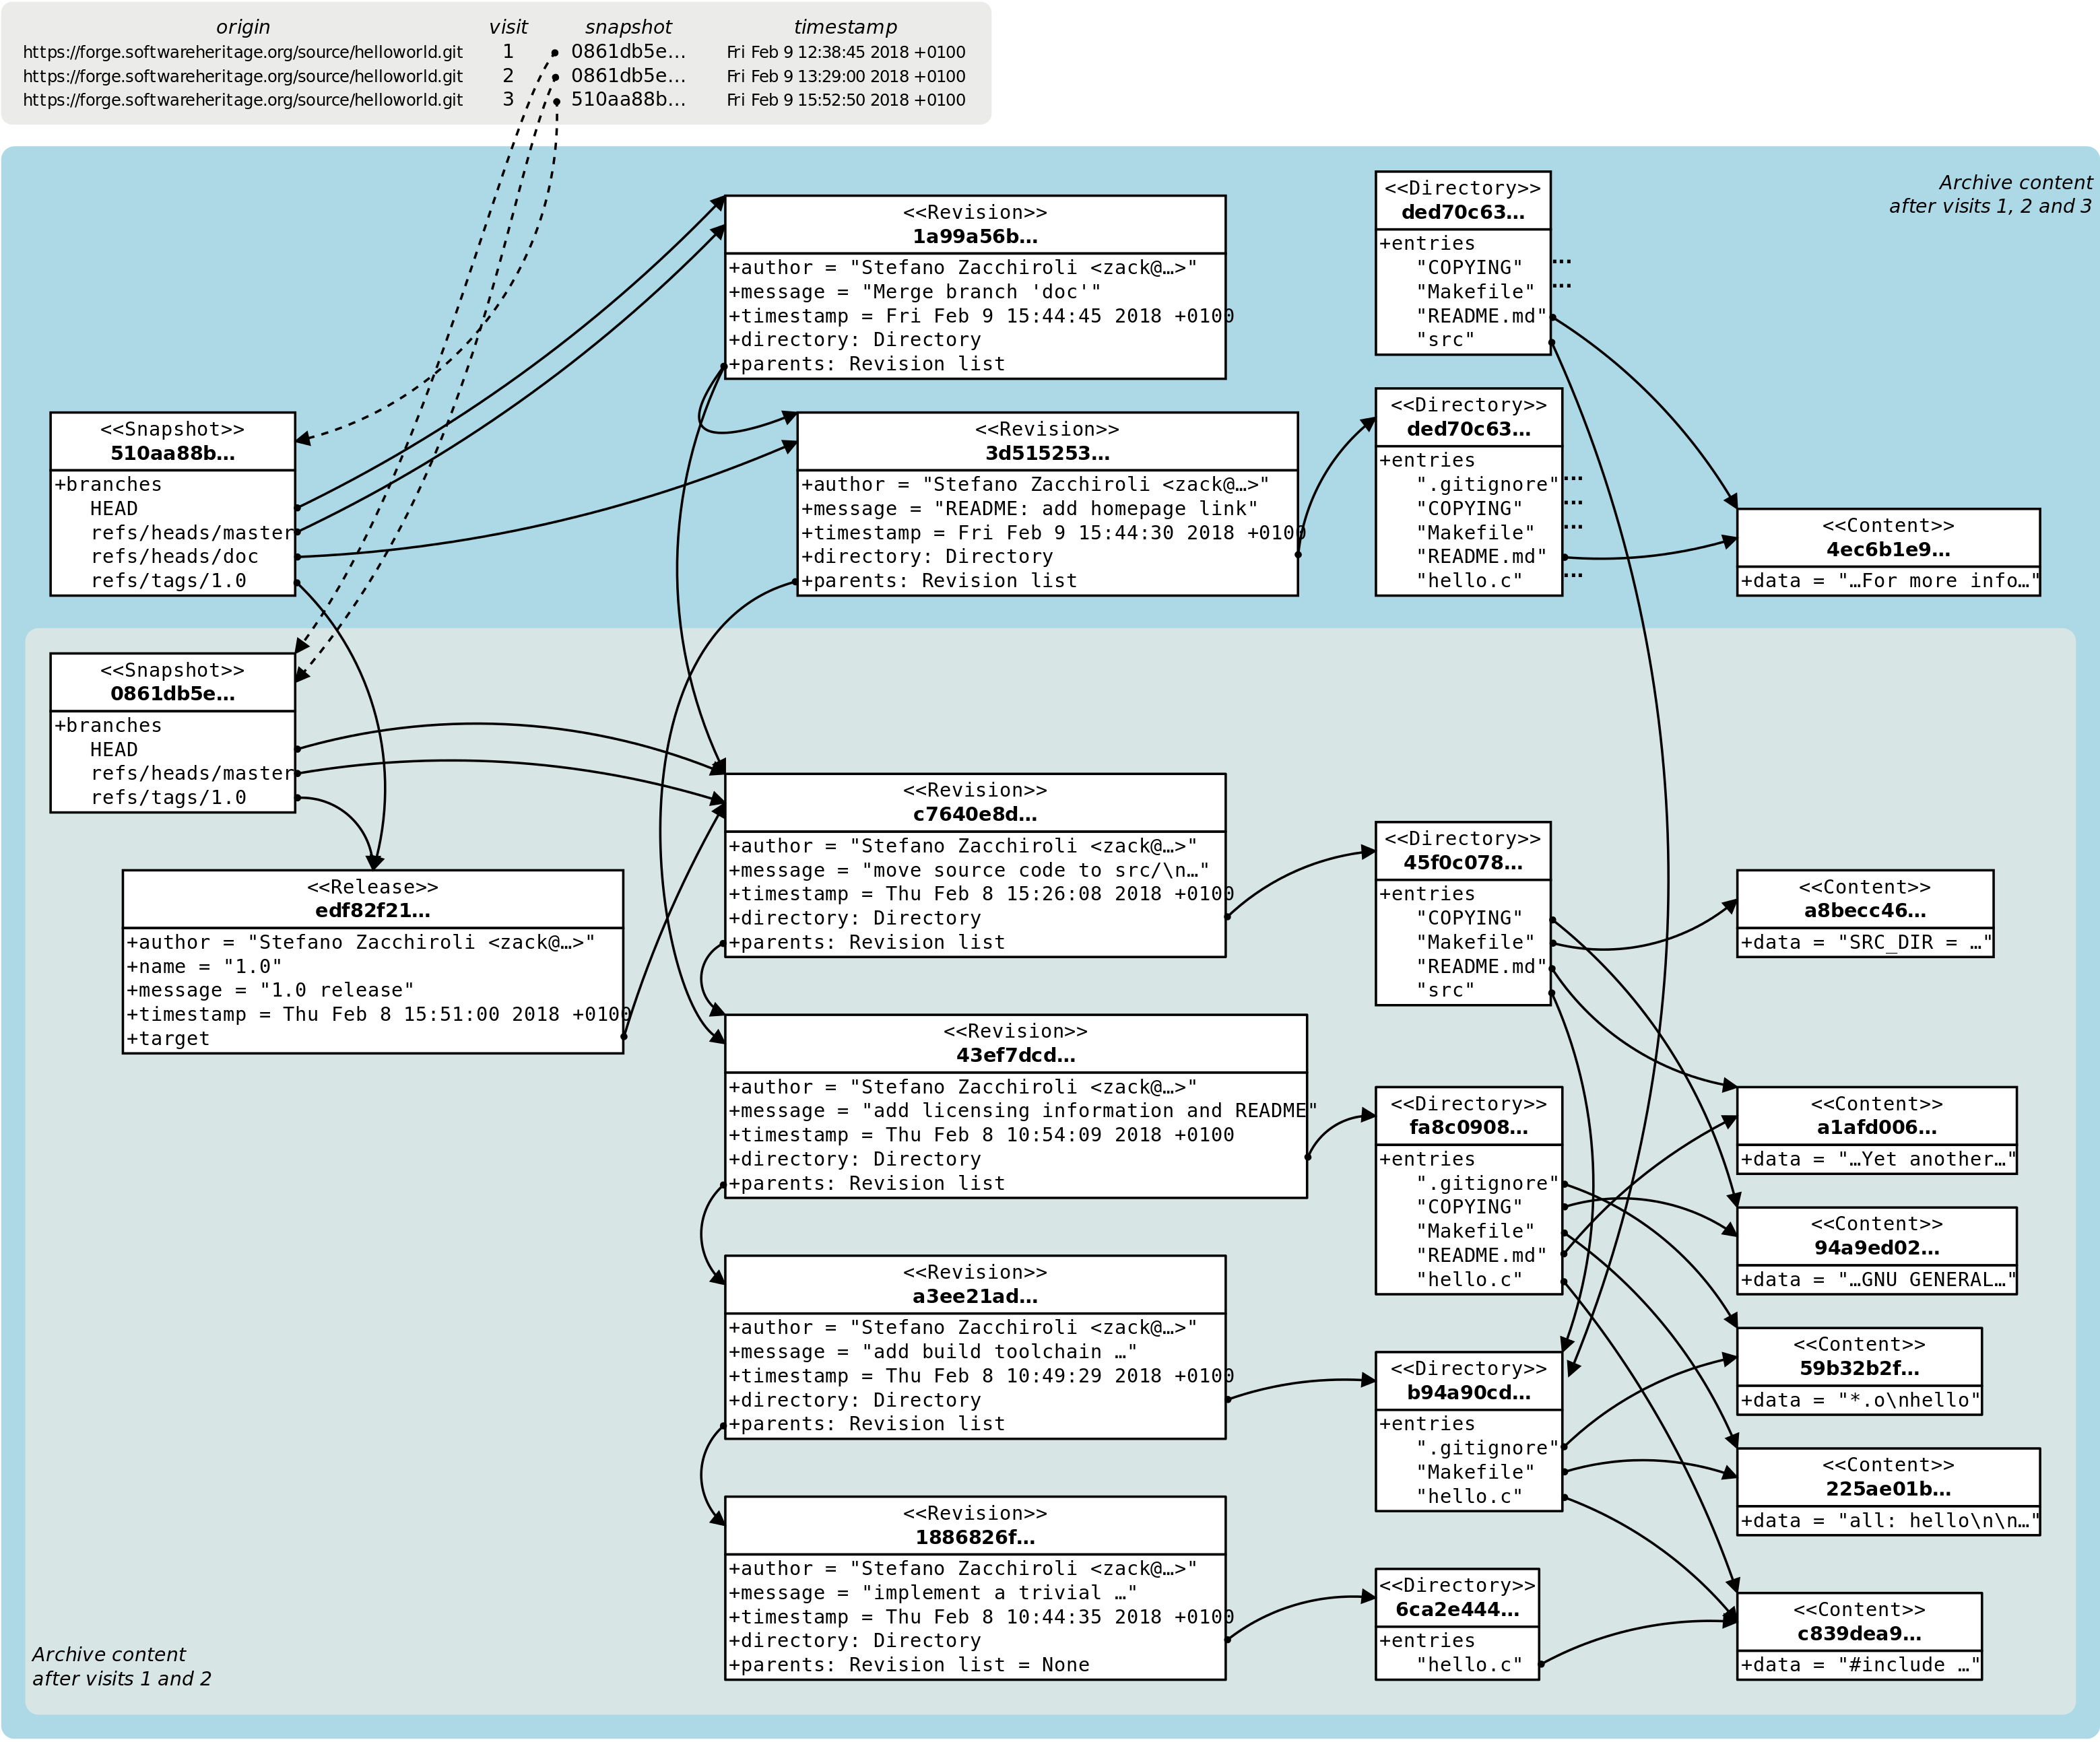
\includegraphics[scale=0.15]{images/swh/data_structure.png}
	\caption{\textbf{Merkel DAG} de \texttt{Software Heritage}\textsuperscript{\citep{swhRevisionNode}}}
	\label{fig:swh_data_structure}
\end{figure}

Le \textbf{Merkel DAG} est composé de noeuds et d'arcs tels que :
\begin{enumerate}
	\item \textbf{noeuds} -- chaque noeud :
	\begin{itemize}
		\item désigne un \textbf{artefact logiciel unique} ;
		\item est identifié par un \textbf{identifieur intrinsèque} désignant un digest cryptographique calculé à partir du noeud et son contenu. Ceci implique qu'un \textbf{software origin} sera ajouté au \textbf{Merkel DAG}, uniquement quand celui-ci ne contient pas déjà un noeud ayant le même identifiant. Cette propriété du \textbf{Merkel DAG} assure une \textbf{déduplication native} à l'archive implanté ;
		\item contient l'ensemble des \textbf{métadonnées} qui lui sont propres (\textit{e.g. messages de commit, estampilles, noms de fichiers, $\dots$}) ;
		\item contient des pointeurs vers les identifiants des \textbf{noeuds enfants} en format canonique.
	\end{itemize}
	\item \textbf{arcs} :
	\begin{itemize}
		\item les \textbf{directories} pointent sur des \textbf{blobs} et d'autres \textbf{directories} ;
		\item les \textbf{revisions} pointent sur des \textbf{directories} et les \textbf{revisions} précédentes ;
		\item les \textbf{releases} pointent sur des \textbf{revisions} ;
		\item les \textbf{snapshots} pointent sur des \textbf{releases} et des \textbf{revisions}.
	\end{itemize}
\end{enumerate}

Un noeud du \textbf{Merkel DAG} désignant une \textbf{revision} est présenté dans la figure \ref{fig:swh_revision_node}. On voit bien l'identifiant intrinsèque du noeud, ainsi que celui du noeud désignant le \textbf{directory racine} pointé par la \textbf{revision}, et celui du noeud désignant la \textbf{revision} précédente. De plus, on voit la date d'ajout, l'auteur, le commiteur, le message et la date du commit de la \textbf{revision}.

\begin{figure}[!ht]
	\centering
	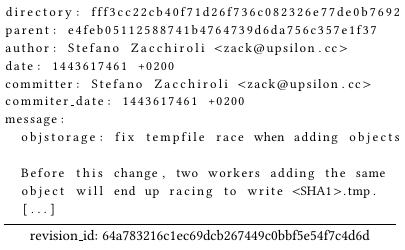
\includegraphics[scale=0.5]{images/swh/revision_node_example.png}
	\caption{Un noeud du \textbf{Merkel DAG} de \texttt{Software Heritage}\textsuperscript{\citep{dicosmoWhyAndHow}}}
	\label{fig:swh_revision_node}
\end{figure}

\subsection{Architecture conceptuelle et flot des données}
\subsubsection{Flot d'ingestion des données}
L'architecture à adopter pour la plateforme doit permettre de \og \textit{crawler} \fg~ une liste de plateformes d'hébergement de code source et d'archiver leur contenu. Pour ce faire, l'équipe de \texttt{Software Heritage} ont adopté une architecture conceptuelle\textsuperscript{\citep{dicosmoWhyAndHow}} divisant la tâche en deux sous-tâches, effectuées respectivement par deux composants de base: le \textit{listing} des plateformes d'hébergement par des \textbf{Listers} et le \textit{loading} de leur contenu au sein de l'archive de par des \textbf{Loaders} (cf. Figure \ref{fig:swh_conceptual_architecture}).

\begin{figure}[!ht]
	\centering
	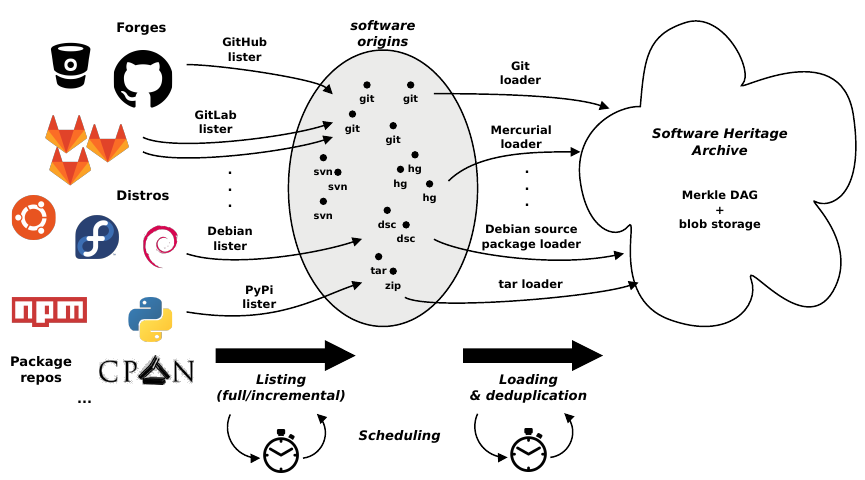
\includegraphics[scale=0.5]{images/swh/conceptual_architecture.png}
	\caption{L'architecture conceptuelle de la plateforme de \texttt{Software Heritage}\textsuperscript{\citep{dicosmoWhyAndHow}}}
	\label{fig:swh_conceptual_architecture}
\end{figure}

\subsubsection{Listing}
Le \textit{listing} d'une plateforme d'hébergement de code source consiste à énumérer les \textbf{software origins} qui lui sont associés (e.g. des dépôts sur \texttt{GitHub} ou \texttt{BitBucket}, des paquets source individuels de \texttt{PyPI} ou \texttt{Debian}, $\dots$). Pour chaque plateforme, un \textbf{Lister} dédié doit être créé afin de \og \textit{mapper} \fg les modèles des \textbf{software origins} vers des modèles équivalents intégrables au sein de l'architecture de \texttt{Software Heritage}\textsuperscript{\citep{dicosmoWhyAndHow}}.

En outre, il existe deux techniques de \textit{listing} :
\begin{description}
	\item [\textit{full listing} :] collecter la liste entière des \textbf{software origins} associée à une plateforme d'hébergement de code, afin s'assurer de n'en rater aucun. Il s'agit d'une technique à utiliser une seule fois initialement, et d'une manière moins fréquente ultérieurement en raison de son aspect chronophage, surtout quand la plateforme est relativement grande.
	\item [\textit{incremental listing} :] collecter uniquement l'ensemble des \textbf{software origins} qui ont été modifiés ou ajoutés depuis le dernier \textit{listing}. Il s'agit d'une technique à privilégier et à utiliser régulièrement, suite au premier \textit{full listing}, pour la mise à jour des noeuds correspondant aux \textbf{software origins} au sein du \textbf{Merkel DAG}.
\end{description}

De plus, il existe deux styles de \textit{listing} :
\begin{description}
	\item [\textit{pull style} :] l'archive consulte régulièrement les plateformes d'hébergement de code en vue de lister leurs \textbf{software origins}. Cette technique est assurée par défaut par les \textbf{Listers} apropriés.
	\item [\textit{push style} :] les plateformes d'hébergement collaborant avec \texttt{Software Heritage}, si proprement configurées, notifient l'archive à chaque modification de leurs \textbf{software origins} associés. Cette technique permet de minimiser le décalage entre la version archivée et la version hébergée d'un \textbf{software origin}.
\end{description}

\subsubsection{Loading}
Le \textit{loading} du contenu des \textbf{software origins} d'une plateforme d'hébergement de code, correspond à l'extraction de leurs \textbf{artefacts logiciels} associés et leur ingestion au sein de l'archive. Pour chaque type de \textbf{software origin}, un \textbf{Laoder} dédié doit être créé afin d'\og \textit{ingérer} \fg les \textbf{artefacts logiciels} et \textbf{snapshots} associés, en assurant la contrainte de déduplication des noeuds au sein du \textbf{Merkel DAG}\textsuperscript{\citep{dicosmoWhyAndHow}} (e.g. un \textbf{Loader} pour chaque gestionnaire de version tels que \texttt{Git} ou \texttt{SVN}, un \textbf{Loader} pour chaque format d'un paquet source tels que \texttt{Debian source packages} ou \texttt{tarballs}, $\dots$).

\subsubsection{Scheduling}
Les tâches de \textit{listing} et de \textit{loading} occurrant régulièrement, un composant permettant de planifier leurs occurrences s'avère ainsi primordial. Il s'agit du composant \textbf{Scheduler}, permettant de \textbf{synchroniser} ces tâches dans une \textbf{queue de tâches asynchrones} opérée par un \textbf{serveur} \texttt{Celery}.

Le \textbf{Scheduler} est implémenté selon les stratégies d'\textit{adaptive scheduling} et d'\textit{exponential backoff}, s'appuyant la notion d'\textbf{actions fructueuses} ou \textit{fruitful actions}. Ces stratégies permettent d'équilibrer entre la mise à jour du contenu de l'archive et la surcharge des plateformes concernées (\texttt{Software Heritage} et les plateformes d'hébergement de code consultées), surtout lors du \textit{loading} des \textbf{software origins} listés associés à une plateforme assez large.

\begin{definition}[\textbf{Fruitful Action}]\mbox{}\\
Une \textbf{action}, désignant une \textbf{tâche périodique à planifier} (\textit{i.e. listing} ou \textit{loading}), est considérée \textbf{fructueuse}	si la visite associée à l'action retourne de \textbf{nouvelles informations} depuis la \textbf{dernière visite} :
\begin{description}
	\item [\textit{fruitful listing} :] lors de la découverte de nouveaux \textbf{software origins} à \og \textit{lister} \fg~ ;
	\item [\textit{fruitful loading} :] lors du changement de l'état d'un \textbf{software origin} consulté depuis la dernière visite.
\end{description}
\end{definition}

\begin{definition}[\textbf{Adaptive Scheduling and Exponential Backoff}]\mbox{}\\
La \textbf{stratégie} d'\textbf{Adaptive Scheduling} permet d'\textbf{augmenter la fréquence} des visites d'une \textbf{action} quand celle-ci est \textbf{fructueuse}, et de la \textbf{diminuer} dans le cas contraire. Le \textbf{taux} de cette augmentation/diminution est spécifié par la \textbf{stratégie} d'\textbf{Exponential Backoff}, indiquant de le \textbf{doubler} en cas d'une \textbf{augmentation} et de le \textbf{diviser par deux} en cas d'une \textbf{diminution}.
\end{definition}

\subsection{L'archive}
% ##Archive
% 1. logical representation: Merkel DAG data structure
% 2. physical storage: different technologies due to the differences in size requirements for storing different parts of the graph

\subsubsection{Stockage des noeuds BLOB de l'archive}
%les IDs, les fichiers
% 3. blob nodes storage:
%   - storage space: occupy the most space as they contain the full content of all archived source code files
%   - storage technology:
%     a. key-value object storage (key = intrinsic identifier of the Merkel DAG node)
%     b. pros:
%       * horizontal scaling: distribution of the object storage over multiple machines -> performance and redundancy
%       * key-value paradigm is very popular among current storage technologies -> easily host copies of the bulk of the archive on premise/public cloud offerings


\subsubsection{Stockage des autres noeuds des archives}
% chemins, repertoires, snapshot, revisions, releases\\
% postgres, etc
% - RDBMS (Postgres):
% 	a. roughly one table per node type
% 	b. key: intrinsic identifier of Merkel DAG node
% 	c. pros:
% 		* horizontal scaling across multiple servers
% 		* master/slave replication and point-in-time recovery -> performance and recovery

\subsubsection{Stockage haché des objets}
% - problem: hash collisions if two different objects hash to the same intrinsic identifier -> risk of storing only one of the node
% - solution: multiple cryptographic checksums with unicity constraints on each of them to detect collisions before adding new software artifact to the archive
% - types of checksums:
% 	a. used: SHA1, SHA256, "salted" SHA1 checksums (in the style of what Git does)
% 	b. in the process of adding: BLAKE2 checksums

\subsubsection{Mise en mirroir des noeuds}
% - change feed:
% 	a. each type of node is associated to a change feed that takes note of all changes performed to the set of objects in the archive
% 	b. persistent
% 	c. the archive is append-only -> under normal circumstances, each feed will only list additions of new objects as soon as they are ingested into the archive
% - pro of using change feeds: ideal for mirror operators -> after a full mirror step, can cheaply remain up to date w.r.t. the main archive

\subsubsection{Politique de rétention}
% - current retention state:
% 	a. two in-house mirrors of the entire object storage
% 	b. a third copy currently being populated on a public cloud
% - retention policy example: each file content must exist in at least 3 copies
% - process: a software component of the archive:
% 	a. keeps track of the number of copies of a given file content and where each of them is
% 	b. periodically swipe all known objects for adherence to the policy
% 	c. when fewer copies than desired exists, additional copies as needed to satisfy the retention policy are asynchronously made by the archiver

\subsubsection{Récupération automatique des objects corrompus}
% - example of an object corruption scenario: storage media decay
% - process: a software component of the archive:
% 	a. periodically checks each copy of all known objects: random selection at a suitable frequency
% 	b. recomputes the intrinsic identifier of each copy and compares it with the known one to verify its integrity
% 	c. in case of a mismatch:
% 		* all known copies of the object are checked on-the-fly again
% 		* assuming one pristine copy is found, it will be used to overwrite corrupted copies -> automatic healing

\subsection{Architecture technique}

\section{Méthodologie}
% Sourceforge sitemap, api\\
% Launchpad api, client\\
% Analyzing the listers (bitbucket, gitlab, github, eclipse, LIRMM, OpenHub, 			Assembla, GNU savannah\\
% heritage, injection de dependances\\
% conclusion: on adoptera une strategie pour definir un lister, loader ou autre\\

\section{Planning Prévisionnel}

\chapter{Conception}
design de la solution proposée (diagrammes + explications)

\chapter{Implémentation}
les technos qu'on a utilisé\\
bibliotheques\\
Outils (e.g. XML parsers)\\
Launchpad client

\chapter{Résultats}
pull request?

\chapter{Conclusion}
\section{Planning final}

\section{Difficultés rencontrées}

\section{Perspectives}

\section{Bilan et apports du TER}
annexes\\
resumés\\
code

\bibliographystyle{unsrt}
\bibliography{mybib}

\end{document}
